\documentclass[12pt]{article}
\usepackage[english]{babel}
\usepackage[utf8]{inputenc}
\usepackage{amsmath, amssymb, amsthm}
\usepackage{graphicx}
\usepackage{hyperref}
\usepackage[margin=.75in]{geometry}
\usepackage{xcolor}
\usepackage{tikz}

\newcommand{\id}{\text{id}}
\newcommand{\od}{\text{od}}

\setlength{\topmargin}{0pt}
\setlength{\headsep}{0pt}
\textheight = 600pt

\title{Graph Theory \\ Homework 18}
\author{Ben Kallus and Josef Komissar}
\date{Due Monday, May 10}

\begin{document}

\maketitle

\medskip\noindent\textbf{11.6} $r(K_{1, 3}, P_3) = 5$.
\begin{proof}
    Note that $r(K_{1, 3}, P_3) > 4$ because of the following counterexample:

    \begin{center} 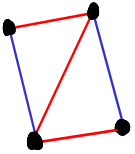
\includegraphics{1.png} \end{center}

    We now show that $r(K_{1, 3}, P_3) \leq 5$.
    Color the edges of $K_5$ red and blue.
    Suppose some vertex has two or more blue incident edges.
    Then the graph has a blue $P_3$ as a subgraph.
    If no vertex has two or more blue incident edges, then some vertex $v$ has less than two blue incident edges.
    Thus, $v$ must have at least three incident red edges, which creates a red claw as a subgraph.

    Thus, $r(K_{1, 3}, P_3) = 5$.
\end{proof}

\newpage\noindent\textbf{11.8} $r(2K_2, 3K_2) = 7$.
\begin{proof}
    The following counterexample shows that $r(2K_2, 3K_2) > 6$:
    \begin{center} 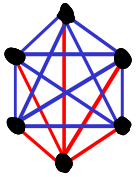
\includegraphics[scale=.65]{10.png} \end{center}
    
    We now show that $r(2K_2, 3K_2) \leq 7$.
    Color the edges of $K_7$ blue and red.
    If any two independent edges are red, then the graph has a red $2K_2$ subgraph.
    Suppose that no two independent edges are red.
    Then, the graph has either all blue edges, its red edges form a triangle, or its red edges form a $K_{1,k}$ for some $1 \leq k \leq 6$.
    Obviously, if the graph has no red edges, then it contains a blue $3K_2$ subgraph.
    Similarly, if the red edges form a $K_{1,k}$, then the vertices that are not in the partite of order 1 form a blue $K_6$, so the graph contains a blue $3K_2$.
    If the red edges in the graph form a triangle, then because all triangles in $K_7$ are symmetric, the following drawing shows that the graph contains a blue $3K_2$ subgraph:
    \begin{center} 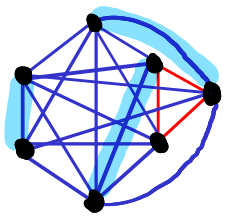
\includegraphics[scale=.5]{11.png} \end{center}
    Thus, $r(2K_2, 3K_2) \leq 7$, so $r(2K_2, 3K_2) = 7$.
\end{proof}

\newpage\noindent\textbf{11.10} $r(P_3, P_3 \cup P_2) = 5$.
\begin{proof}
    Note that $r(P_3, P_3 \cup P_2) > 4$ because of the following counterexample:
    \begin{center} 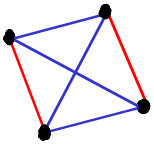
\includegraphics{5.png} \end{center}
    We now show that $r(P_3, P_3 \cup P_2) \leq 5$.
    Color the edges of $K_5$ blue and red.
    If there is only one red edge, the because all edges in a complete graph are symmetric, the image below shows that the graph has a blue $P_3\cup P_2$ subgraph.
    \begin{center} 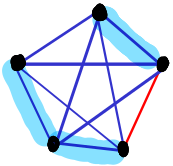
\includegraphics{6.png} \end{center}
    If there are exactly two nonadjacent red edges, then because every pair of nonadjacent edges in a complete graph is symmetric, there is a blue $P_3\cup P_2$ subgraph as seen in the image below:
    \begin{center} 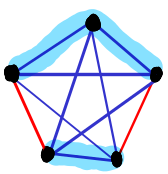
\includegraphics{7.png} \end{center}
    If there are three or more red edges, two of them must be adjacent by the Pigeonhole principle, so the graph contains a red $P_3$ subgraph.
    Thus, $r(P_3, P_3 \cup P_2) = 5$.
\end{proof}

\newpage\noindent\textbf{11.12} $r(P_4, P_4) = 5$.
\begin{proof}
    The following counterexample shows that $r(P_4, P_4) > 4$:
    \begin{center} 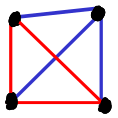
\includegraphics{8.png} \end{center}
    
    We now show that $r(P_4, P_4) \leq 5$.
    Color the edges of $K_5$ red and blue.
    Let $v$ be a vertex in this graph with neighbors $u, w, x$ and $y$.
    Suppose without loss of generality that $uv, wv$ and $xv$ are all red.
    Suppose without loss of generality that $uw$ is red, as well.
    Then, the graph contains the red $P_4$ induced by $\{u, w, v, x\}$.
    Now, suppose that all of $uw, ux, wx$ are blue.
    If $uy$ is blue, then $\{y, u, x, w\}$ induces a blue $P_4$.
    If $uy$ is red, then $\{y, u, v, w\}$ induces a red $P_4$.
    By a symmetric argument, if there is a vertex with three or more incident blue edges, then the graph contains a monochromatic $P_4$.
    Suppose that every vertex in the graph is incident to exactly 2 red edges and 2 blue edges.
    Note that the construction of any such graph would begin with a graph isomorphic to the one shown below:
    \begin{center} 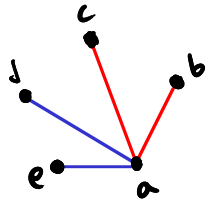
\includegraphics[scale=.7]{9.png} \end{center}
    No matter the color of the edge $bd$, a monochromatic $P_4$ will be created.
    Thus, $r(P_4, P_4) = 5$.
\end{proof}

\newpage\noindent\textbf{11.16} $r(K_3, K_n) \leq {n+1 \choose 2}$ for all $n \geq 2$.
\begin{proof}
    Observe that $r(K_3, K_2) = \max\{|V(K_3)|, |V(K_2)|\} = 3$.
    Inductively assume that $r(K_3, K_{n-1}) \leq {n \choose 2}$ for some $n \geq 3$.
    Consider a coloring of $K_{n + 1 \choose 2}$.
    Let $u$ be a vertex in $K_{n + 1 \choose 2}$.
    Then, by Pascal's Identity, $\deg(u) = {n \choose 2} + n - 1$.
    Thus, by the Pigeonhole Principle, $u$ is incident to either at least ${n+1 \choose 2}$ blue edges or at least $n$ red edges.
    Suppose that $u$ is adjacent to at least ${n+1 \choose 2}$ vertices via blue edges.
    Then, among those vertices, there is either a red $K_3$ or a blue $K_{n-1}$.
    If there is no red $K_3$, there must be a blue $K_{n-1}$ by the inductive assumption.
    Since $u$ is connected to each of these vertices via a blue edge, we have identified a blue $K_n$.
    Now, suppose that $u$ is adjacent to at least $n$ vertices via red edges.
    Then, if any of those vertices are connected via a red edge, then the graph has a red $K_3$.
    If all of these vertices are connected with blue edges, then the graph has a blue $K_n$.
    Thus, by induction, $r(K_3, K_n) \leq {n+1 \choose 2}$.
\end{proof}

\newpage\noindent\textbf{LASTLY} The Book is Erdös's hypothetical transfinite book containing all the best possible proofs that are ``elegant and perfect."

\end{document}

